% !TeX root = ../main.tex

\chapter{Related Work}\label{chapter:Related Work}

This chapter surveys previous work in the automatic assessment of vulnerabilities. We will see how their approach differs from what we have done, the viability of their work, in respect to what we have learned in this thesis. Moreover, we will see if what they have done matches in some way what we have also done, and try to mirror or approximate their ideas to what we have researched and developed.

\section{MACKE's ranking of vulnerabilities}

As mentioned previously in 3.1.3, MACKE is a compositional symbolic analysis, of which we have talked extensively throughout this thesis, but only emphasising on its first two steps, while leaving the third one completely on the sidelines. The reason being, it has its own severity assessment tool, which is not automized, and the results have to be parsed to get them. Nonetheless, the research done in \parencite{ognawala} is relevant to us because of its closeness to the topic -- assessing the severity of vulnerabilities found through symbolic execution -- at hand.

In \parencite{ognawala} 2.2.3 "Ranking the Vulnerabilities" it is mentioned that :
\\\\
\enquote{\texttt{A thorough compositional analysis for finding low-level
		vulnerabilities is more useful when there is a process to
		prioritize those vulnerabilities. After consulting with our
		industry partners, we decided to implement in our framework
		an interactive procedure to assign severity scores to
		vulnerable functions that are found in the analysis stages
		of MACKE. This severity score is based on the functions
		described below (with their intuition), and a weight (impact
		factor) between 1 and 5 associated with each function (i) The function len chain(f) returns a natural number representing
		the depth of function hierarchy through which a
		vulnerability in f might be exploited. It has the impact factor
		L. If a function can be exploited through a long hierarchy,
		it’s more likely somebody forgot to sanitize the exploit input.
		(ii) The function is int(f) returns a boolean according to
		whether the function f is an exposed interface or not. It has
		the impact factor I. Vulnerability in an exposed interface,
		such as the main function, is easily exploitable and must
		be fixed with higher priority. (iii) The function vuln inst(f)
		returns the number of distinct \\ instructions that were found
		to contain a vulnerability and has the impact factor N. More
		vulnerabilities strongly indicates a missing input sanitization
		check somewhere in the function. (iv) The function
		d interface(f) returns the proximity (length of the nested function
		chains) of the function to an exposed interface and has
		the impact factor D. A vulnerable function closer to an exposed
		the interface may be easier to exploit. (v) The function
		is an outlier(f) returns a boolean depending on whether the
		number of vulnerable instructions found (Section 2.2.1) is
		much greater than the average number of vulnerable instructions
		per function in the program. The intuition behind this
		is the same as that for vulnerable inst(f). It has the impact
		factor O.
		We formulated the above functions with our industry partners
		and, based on our combined intuitions on the programs
		that we analyzed, we used the following function, s, to calculate
		the total severity value:
		\\\\
		s(f) = L * len chain(f) + I * is int(f) + N * vuln inst(f)
		+ D * d interface + O * is outlier(f)
		\\\\
		Functions with higher severity scores are, in our view, more
		vulnerable to attacks. The specific values for the impact
		factors are also, as the function s itself, dependent on the
		context of development and vulnerability analysis, as we
		clarify once more in Section 3.
		As a final presentation step, MACKE color codes the
		ranges of severity scores for all functions in the program
		and displays the call graph, with function and instruction
		level details of the test cases that cause a vulnerability to be exposed with compositional \\analysis.}}
\\\\

To decompose what has been done by them is extremely important, and putting it into perspective, we can see where we align and were our ideas deviate and see how this area of research could be improved upon in the future.

\subsection{MACKE's severity assessment}

As it was previously quoted, they use a formulaic approach to find the severity of a vulnerability. They used the following formula : 
\\\\
s(f) = L * len chain(f) + I * is int(f) + N * vuln inst(f)
+ D * d interface(f) + O * is outlier(f)
\\\\
Decomposing the formula is of great importance. Knowing that s(f) is the severity of a given function s, we continue to evaluate the variables involved in the formula.

\begin{itemize}
	\item L - Impact factor of len chain(f).
	\item len chain (f) - The depth of function hierarchy through which f can be exploited.
	\item I - Impact factor of is int (f).
	\item is int(f) - Whether the function is an interface or not.
	\item N - Impact factor of vuln inst (f).
	\item vuln inst(f) - Amount of vulnerabilities found in a function
	\item D - Impact factor of d interface(f).
	\item d interface (f) -  Proximity of the function to an exposed interface.
	\item is an outlier(f) - If a number of vulnerabilities found in the function is greater than the average for the program.
\end{itemize}

\begin{figure}[!htb]
	\caption{MACKE's severity ranking framework using (L=3,I=5,N=2,D=4,O=1)}
	\centering
	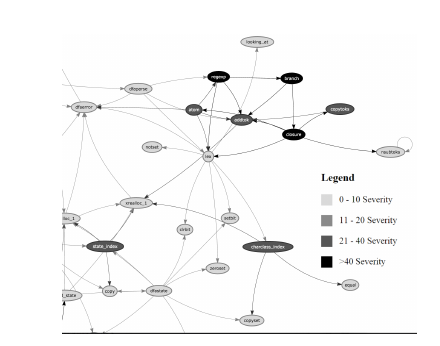
\includegraphics[width=0.7\textwidth]{macke_framework}
\end{figure}

First, it is worth mentioning that their use of impact factors differs from our approach, but it is clearly seen as to what it was done. The reasoning behind it was to disregard these values when they were not found, thus being multiplied by 0 and therefore not being taken into account.

\subsubsection{L and len chain (f)}

When looking at L * len chain(f) we can see that it is doing exactly the same we are doing in our framework, which we called "Macke bug chain length".

They do not go into the intricacies of how it was done, but we can deduce that they are using MACKE's phase 2 values to come up with a chain of function calls, to know how long it is. L is its impact factor.

\subsubsection{I and is int(f)}

These values tell us how far a function is an entry point or "interface", which we do not use since we used the external node of every call graph as our interface for all of our measurements. Therefore calculating this value in our framework would have been futile (only one node would have been a 1).

\subsubsection{N and vuln inst(f)}

This value yet again aligns with another value used in our framework, this time with "Macke bug chain length". What vuln inst(f) does is return how many vulnerabilities were found by MACKE in that specific function. N is its impact factor.

\subsubsection{D and d interface(f)}

This value is identical to one we also use:"distance to interface". It has the same meaning, and they do the calculation the same way, the only difference being that they calculated several interfaces instead of just one as is in our case (using the external node, always). D is its impact factor.

\subsubsection{is outlier(f)}

This value, being a boolean like many others, but without an impact factor, depicts only whether the function has more vulnerabilities than the average found for the entire program. This we did not use, nor consider, though it can have some importance. The main reason why this didn't cross our minds is that generating an average could be misleading sometimes, if the values were generally low, and just a few functions had anything above it, they would have been counted as outliers, which would have impacted the severity, when in truth, it could be that it is just one vulnerability spreading throughout the function. MACKE would find this as several vulnerabilities, though for example, something as simple as the sanitization of a variable could go a long way between having 5 vulnerabilities in a function and having 0, which does not mean it is more critical than another function that has a buffer overflow that grants root privileges.

\subsubsection{MACKE's severity assessment}

The severity retrieved from using the aforementioned s(f) is a number, which can be a number from 0 to > 40, which can fall into several categories as shown in Figure 5.1 \parencite{ognawala}. The problem with this approach, in our minds, is that it is not standardized. While MACKE might be using these values, and color coding, it will differ greatly from what the industry is doing, therefore rendering these results useless when given to someone who is clueless to the idea of symbolic execution, not to say MACKE. We strongly believe that their approach was one in the right direction, and has given us ideas, which we used as building blocks for this thesis. Our work would not have been possible without this previous knowledge.

\subsubsection{What can we take away?}

The most important thing to be taken away from this research is that it corroborated our approach in regards to the node attributes and MACKE results used in our interface. We believe that we have taken a step in the right direction by using a similar approach, but assessing the severity in terms of the biggest vulnerability assessment standard in the world, CVSS\parencite{cvss3}.

\section{A Novel Automatic Severity Vulnerability Assessment Framework}

In \parencite{novelty} a new framework named by its developer "Automatic Security Vulnerability Assessment Framework" or ASVA, aims to resolve the problems that Quantitative Vulnerability Assessment Standards (QVAS) such as CVSS have.

The focus of this paper is mainly on network security, rather than general vulnerabilities, though the proposed framework is generic. Furthermore, the framework has taken CVSS into account and tried to build upon it.

\subsection{How to improve upon current QVAS?}

They mention how CVSS, being an objective, authoritative, and transparent quantitative vulnerability assessment standard (QVAS), is still difficult to implement in all projects, their reasons being some of the following:

\begin{itemize}
	\item The number of vulnerabilities grows ever so larger in all software projects, and adding CVSS scores only adds to the complexity of filing, fixing and deploying vulnerabilities.
	\item There is not a huge collection of bugs in vulnerability databases because of it -- CVSS -- being so recently adopted.
	\item The categorization of certain base scores of CVSS can be subjective, depending on who is making the assessment.
\end{itemize}

What it is proposed in this paper \parencite{novelty}, is something similar to what we have developed: not a new QVAS, but the introduction of an application process of an existing QVAS, which in our case was CVSS.

The main methodology used to get the base scores would be by using Text Mining. With their tool ASVA, they would compute the severity values and ranks of vulnerabilities using other QVAS, when there was a lack of information.

Interestingly, they also used the NVD database, along with three non-NVD Databases. They also introduce three dimensions (accuracy, coverage rate, and dispersity) to analyze the results, results show that the accuracy of severity rank is 90.1\% and the dispersity
is perfect. They then go on to explain the reasoning behind errors in the vulnerability assessment, which are all related to machine learning.

\subsection{Pipeline of the ASVA framework}

The following is an abstract of the explanation of each step given directly from the author in \parencite{novelty} and shown in Figure 5.2:

\begin{itemize}
	\item Stage I includes Step 1. The task of Stage I is acquiring and cleansing data. We can obtain the one-to-one corresponding vulnerabilities between Auxiliary VDB and Target VDB as Training Set, and obtain the rest vulnerabilities of Target VDB as Test Set.
	\item Stage II includes Step 2. The task of Stage II is determining the classification metrics. ASVA contains three modes, all of them have different metrics.
	\item Stage III includes Step 3, Step 4 and Step 5. The task of Stage III is classifying metrics with Text Mining and obtaining the values of metrics.
	\item Stage IV includes Step 6 and Step 7. The task of Stage IV is assigning values of metrics to formulas of the QVAS and computing the severity values and severity ranks of vulnerabilities.
\end{itemize}

\begin{figure}[!htb]
	\caption{The process of ASVA}
	\centering
	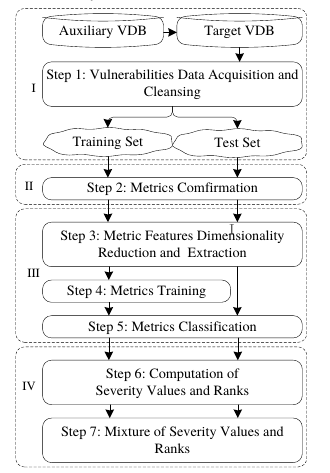
\includegraphics[width=0.7\textwidth]{asva_pipeline}
\end{figure}

Since our thesis does not touch on the topic of Text Mining, nor is its intention, we will focus on the matter at hand which is the extraction of the results, in this case, the CVSS scores. In this regard, this tool uses, unfortunately, CVSS 2.0, which had a much more simplistic way of assigning base scores but also was not so accurate. 

With that in mind, we can tell that while they used a similar approach to ours (e.g using NVD as the main vulnerability database used because of its reliability among other attributes, and their fixation on using CVSS as the main standard), it is clearly they took a more statistical approach, rather than an algorithmic one, such as the one we did.

They mention that when their coverage rate is 100\%, the rank -- base score -- accuracy is 82.5\%, but when the coverage is 76\% the accuracy goes up to 90.1\%. We believe that this has to do with the statistical approach that they took, and how based on a smaller amount of words analyzed, the hit chance is higher.

\subsection{Is ASVA an improvement over our current framework}

Their approach is extremely interesting, and the way they went about predicting the CVSS base scores by "cleansing" as they mentioned in \parencite{novelty}, and then checking for patterns is noteworthy, and something we had not considered. Nonetheless, we do not believe that their platform is better, nor worse, but complementary.

The main reasoning behind it is that just parsing through the text, as explained in this paper is not enough since they remove too much context when cleaning the text. What if a single digit, is removed, and it was an assignment that leads to a vulnerability, or if a function called was disregarded when cleansing the source code.

It has been shown throughout this thesis that the relationship between functions, the vulnerabilities found in them, and their neighboring functions are of extreme importance when piecing together the CVSS score of a function.

Therefore, we can say that while this was an extremely good approach, and their results are outstanding, it still lacked the precision, and the right approach for it to be adopted, not to mention the use of CVSS 2.0, which has already been phased out in favor of a new and much-improved version. Furthermore, combining the work from ASVA and our approach could yield an even better result, and we would strongly encourage future work to take both approaches into consideration since both cover the same problem from a different angle.


